TTT

We believe that the design of \CEU make a good tradeoff...

ok on embedded systems

Therefore, our current work with \CEU focus on three main goals:

\begin{itemize}
\item Overcome the limitations of synchronous languages.
\item Become a multi-purpose language.
\item Attract new users.
\end{itemize}

The first...

The second...

\section{Asynchronous execution}

The synchronous computation model of \CEU has some inherent limitations:
%
\begin{itemize}
\item Time-consuming operations break the zero-delay hypothesis of reactions.
      Therefore, \CEU has no support for unbounded loops and blocking C calls 
      (e.g. reading from a socket).
%
\item Input generation is external to the program, making it difficult for a 
      program to simulate its own execution (e.g., for testing purposes).
%
\item Real parallelism is difficult for two reasons:
      the semantics of \CEU is deterministic,
      and the stackless implementation for trails hinders data localization 
      (everything is ``static'').
\end{itemize}

These problems are inherent to the synchronous model and trying to fight them 
by tweaking the language would be a mistake.
%
Our approach is to add support for \emph{asynchronous blocks (asyncs)}, with 
the additional features:
%
\begin{itemize}
\item Can contain unbounded loops.
\item Can make blocking C calls.
\item Can emit input events.
\item Can be parallelizable.
\end{itemize}

Although \emph{asyncs} share the same syntax with \CEU for convenience, they 
can be understood as another language running inside \CEU.
%
In fact, they look much more like $C$ and cannot contain parallel compositions, 
awaits, internal events, finalization blocks, or any synchronous primitive that 
characterizes \CEU.
%
The translation below describes the execution of an \emph{async} from the point 
of view of the synchronous semantics of \CEU:

\begin{figure}[h!]
\begin{minipage}[t]{0.44\linewidth}
\begin{lstlisting}
// asynchronous block
par/or do
    <sync code>
    async do
        <async code>
    end
    <sync code>
with
    <sync code>
end
\end{lstlisting}
\end{minipage}
%
\begin{minipage}[t]{0.56\linewidth}
\begin{lstlisting}
// synchronous interpretation
par/or do
    <sync code>
    emit OUT$_i$;  // spawns <async code>
    await IN$_i$;  // rejoins from <async code>
    <sync code>
with
    <sync code>
end
\end{lstlisting}
\end{minipage}
\end{figure}

In the interpretation, the \code{emit OUT$_i$} makes a non-blocking request to 
start the asynchronous code and is immediately followed by a corresponding 
\code{await IN$_i$}.
%
The \emph{async} runs detached from the \CEU program, which remains responsive 
in the second trail.
%
Once the \emph{async} terminates, it signals \code{IN$_i$} to \CEU (just like a 
normal external event), awaking the first trail.
%
If the second trails terminates before, the \CEU runtime sends an aborting 
signal to the detached \emph{async} (which will never awake the first trail).

Figure~\ref{lst.async.2} shows the implementations in \emph{pthreads} and \CEU 
for a program that makes two heavy calculations in parallel.
%
The \code{par/and} spawns two \emph{asyncs} in parallel, only rejoining after 
they both terminate.
%
The running times in the two implementations are the same, in a duo-core CPU, 
yielding 175\% CPU usage.
%
In terms of implementation, \CEU maps an \emph{async} into a \emph{pthread}, 
using the stack to hold memory and improve data localization.

\begin{figure}[t]
\begin{minipage}[t]{0.37\linewidth}
\begin{lstlisting}
// heavy calculation
void calc () {
 int ret = 0;
 int i, j;
 for (i=0;i<50000;i++)
  for (j=0;j<50000;j++)
   ret += i + j;
 printf("%d\n", ret);
}
\end{lstlisting}
\end{minipage}
%
\begin{minipage}[t]{0.35\linewidth}
\begin{lstlisting}
// pthreads
void main () {
 pth_t t1, t2;
 pth_create(&t1,calc);
 pth_create(&t2,calc);
 pth_join(t1);
 pth_join(t2);
 exit(0);
}


// Time:
// # 17.39s user
// # 175% cpu
\end{lstlisting}
\end{minipage}
%
\begin{minipage}[t]{0.26\linewidth}
\begin{lstlisting}
// Ceu
par/and do
  async do
    _calc();
  end
with
  async do
    _calc();
  end
end

// Time:
// # 17.38s user
// # 175% cpu
\end{lstlisting}
\end{minipage}
\rule{14cm}{0.37pt}
\caption{ A heavy calculation in \CEU with \code{async} blocks.
{\small %\textmd{
}%}
\label{lst.async.2}
}
\end{figure}

\subsection{Simulation}
\label{sec:ceu:simul}

Simulation is an important aspect in cross-compiling platforms, such as 
embedded systems.
It is usually employed to test applications before deploying them on the target 
platform.
%However, simulators are usually inaccurate, varying from platform to platform, 
%and may also require additional knowledge to operate.
%
\CEU can simulate programs in the language itself, not depending on external 
tools.
Given that \emph{asyncs} are allowed to emit input events towards the 
synchronous side of the program, it is easy to simulate and test the execution 
of programs with total control and accuracy with regard to the order of input 
events---all is done with the same language and inside the programs themselves.

\begin{figure}[t]
\begin{minipage}[t]{0.40\linewidth}
\begin{lstlisting}
input int START;
var int v = await START;
par/or do
   loop do
      await 10min;
      v = v + 1;
   end
with
   await 1h35min;
end
\end{lstlisting}
\end{minipage}
%
\begin{minipage}[t]{0.50\linewidth}
\begin{lstlisting}[numbers=left,xleftmargin=-0.5em]
par/or do
   <...> // CODE (in the left)
   _assert(v == 19);
with
   async do
      emit START => 10;
      emit 1h35min;
   end
   _assert(0);
end
\end{lstlisting}
\end{minipage}
\rule{14cm}{0.37pt}
\caption{
A program in the left with a corresponding simulation template in the right.
{\small %\textmd{
}%}
\label{lst.simul}
}
\end{figure}

Suppose we want to simulate the execution of the program in the left of
Figure~\ref{lst.simul}, which initially awaits the input event $START$ (line 2) 
and then increments $v$ every $10$ minutes (lines 4-7) during $1$ hour and $35$ 
minutes (line 7).
%
To test this code, we simulate the occurrence of the event $START$ and the 
passage of \code{1h35min} in a parallel trail, as shown in the right of
Figure~\ref{lst.simul}.
%
The original code remains unmodified and is simply pasted into the template 
(line 2), which runs the simulation in parallel.
%
Note that with a deterministic semantics, a program outcome in \CEU depends 
solely on the events it receives from the environment.
%
The sequence of execution for the simulation is as follows:

{\small
\begin{enumerate}
\setlength{\itemsep}{0pt}
\item The original code initially awaits the event \code{START} (line 2, code 
in the left).
\item The \code{async} (lines 5-9, right) begins, emits \code{START=10} (line 
6, right) and is suspended (synchronous code always have higher priority).
\item The original code resumes and awaits \code{10min} and \code{1h35min} in 
parallel trails (lines 5 and 9, left).
\item The \code{async} resumes and signals that \code{1h35min} has elapsed 
(line 7, right).
\item The original code completely reacts to that: the loop iterates exactly 
$9$ times (lines 4-7, left) before the trail awaiting \code{1h35min} resumes 
(line 9, left) and terminates the innermost \code{par/or}.
The assertion test (line 3, right) executes and terminates the program 
successfully.
The other assertion test (line 9, right) never executes.
\end{enumerate}
}

\begin{comment}
With the proper tools, this integration can be made even simpler (e.g. we 
developed a framework to run tests for the implementation of \CEU{} with 
hundreds of programs and test cases defined in separate).
\end{comment}

It should be clear from the example that simulation does not test true I/O, 
only the program behavior given an arbitrary input sequence.
For instance, the simulation does not take $1$ hour to complete, but actually a 
negligible time.
Also, simulation can be employed---with the exact same behavior---in the 
developing platform or in the target platform.

\begin{comment}
TTT: conclusion?
\subsection{GALS execution}
\label{sec:ceu:gals}

\CEU{} complies with the GALS (\emph{globally asynchronous, locally 
synchronous}) model of computation, which states that local activities run 
synchronized with a common clock, while global activities run with independent 
clocks.
The \emph{globally asynchronous} part of \CEU{} is restricted to external input 
events, $C$ code, and asynchronous blocks, while the \emph{locally synchronous} 
part of \CEU{} extends to all other primitives, such as parallel compositions, 
variable manipulation, and internal events.

The temporal analysis of \CEU{} discussed in Section~\ref{sec:ceu:det} ensures 
that only the locally synchronous part of programs is deterministic.
Therefore, \CEU{} is not an absolutely deterministic language, that is, the 
behavior of programs may vary from execution to execution.

However, nondeterminism in \CEU{} is exclusively a consequence of globally 
asynchronous execution.
For instance, the program in Figure~\ref{lst:ceu:gals} is nondeterministic, 
given that the \code{async} runs for an undetermined time, and may terminate 
before or after the statement \code{await~1s}.
Even so, the \CEU{} compiler does not complain about nondeterminism, because 
the assignments cannot run concurrently.

\begin{figure}[h]
\rule{15cm}{0.37pt}
{\small
\begin{verbatim}
        int ret;
        par/or do
            async do
                ...     // a long computation
            end
            ret = 1;
        with
            await 1s;
            ret = 2;
        end
        return ret;
\end{verbatim}
}
\caption{ The assignments never run concurrently.
\label{lst:ceu:gals}
}
\end{figure}

Note that for simulation purposes, the asynchronous execution can be entirely 
guided by synchronous code, making programs fully deterministic.
For instance, the simulation example of Figure~\ref{lst:ceu:simul:2} can be 
repeated many times, with the exact same behavior.
\end{comment}

\section{Abstractions with ``organisms''}
\label{sec.orgs}

Applications frequently require multiple instances of an abstraction to coexist 
during runtime.
%
%Code reentrancy avoids duplicating code to save ROM, i.e., the same code is 
%shared among instances, which only differ on their data and
%point of execution.
%
In traditional multi-threaded systems, code reentrancy is achieved with 
function declarations that are executed with different stacks and instruction 
pointers.
In object oriented languages, a \emph{class} encapsulates methods and 
properties, and can be instantiated as objects.

In \CEU, we designed an hybrid approach, which combines trails and objects in 
the so called \emph{organisms}.
An organism class is composed of an \emph{interface} and a single \emph{body}.
The interface exposes public variables and internal events that other organisms 
can access.
The body of a class is equivalent to a trail, with all presented functionality 
provided by \CEU, such as parallel compositions, $C$ calls, timers, etc.
An organism is instantiated by declaring a variable of the desired class, and 
its body is automatically spawned in parallel with the enclosing block.

Figure~\ref{lst.orgs} illustrates the use of organisms in \CEU, with an 
application that blinks two LEDs in parallel.
%
The code in the left defines the \code{Blink} class (lines 1-11) exposing the 
\code{led} and \code{freq} variables to be configured by the application (lines 
2,3).
It then initializes to instances (lines 13-16 and 18-21), which start to 
execute their bodies immediately.
%
Once the enclosing block terminates (line 23), both organisms are aborted and 
all memory can be reused.
%
The translation code in the right shows how the organisms bodies are expanded 
to run in a \code{par/or} together with the enclosing block body that 
initializes them (lines 4-8).
The translation is illustrative, i.e., the code is not actually duplicated to 
save memory.
Note that in the expansion, the bodies of the organisms are followed by 
\code{await~FOREVER} (lines 16,24), meaning that only the enclosing block can 
terminate the \code{par/or}.
Note also that the block body runs first and properly initializes the organisms 
before they are spawned, simulating the constructors of organisms.

\begin{figure}[t]
\begin{minipage}[t]{0.45\linewidth}
\begin{lstlisting}
class Blink with
   var int led;
   var int freq;
do
   loop do
      _on(this.led);
      await (this.freq)s;
      _off(this.led);
      await (this.freq)s;
   end
end

var Blink b1 with
    this.led  = 0;
    this.freq = 2;
end;

var Blink b2 with
    this.led  = 1;
    this.freq = 4;
end;

await 1min;
\end{lstlisting}
\end{minipage}
%
\begin{minipage}[t]{0.48\linewidth}
\begin{lstlisting}[numbers=left,xleftmargin=1em]
var _blink_t b1, b2;

par/or do
   b1.led  = 0;
   b1.freq = 2;
   b2.led  = 1;
   b2.freq = 4;
   await 1min;
with
   loop do
      _on(b1.led);
      await (b1.freq)s;
      _off(b1.led);
      await (b1.freq)s;
   end
   await FOREVER;
with
   loop do
      _on(b2.led);
      await (b2.freq)s;
      _off(b2.led);
      await (b2.freq)s;
   end
   await FOREVER;
end
\end{lstlisting}
\end{minipage}
\rule{14cm}{0.37pt}
\caption{ ``Two blinking LEDs'' using organisms.
\label{lst.orgs}
}
\end{figure}

In contrast with objects, note that \CEU organisms are not global entities and 
do not use the heap for memory.
Instead, they are bounded to the scope they are declared, and all memory is 
statically allocated, just like \CEU does with standard local variables.
When an organism goes out of scope, the same automatic bookkeeping of 
\code{par/or} compositions holds, all internal trails are aborted and 
finalization blocks execute (if any).
Hence, the ``garbage collection'' for data and code memory in organisms is 
efficient and static.
%
Methods in \CEU can be simulated by exposing internal events in the class 
interface and all safety guarantees related to bounded memory and execution 
also apply to organisms.

\subsection{Dynamic allocation}

\subsection{New applications}

\begin{figure}[t]
\centering
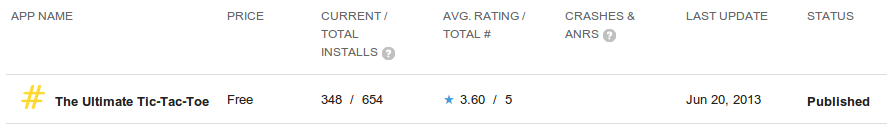
\includegraphics[scale=0.45]{play.png}
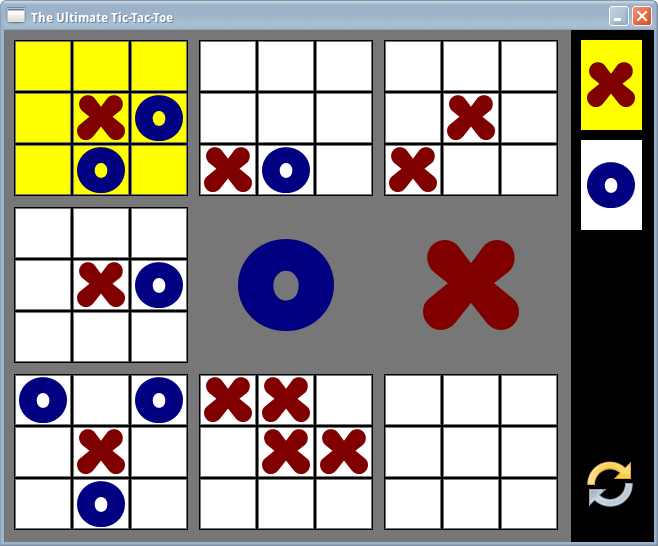
\includegraphics[scale=0.55]{scX.png}
\rule{14cm}{0.37pt}
\caption{ A graphical application in \CEU using the SDL binding.
          The game is published in the ``Android market''.
\label{lst.orgs}
}
\end{figure}

GUI natural
require abstractions, buttons, menus, containers, etc.

- SDL rects
- tic-tac-toe
- networked multi-player game


- nesting
    - data
    - events
    - listeners
    - compositions

- both have an interface
- fields / methods

- fields / internal events
- public fields are ok because reliable shared memory

- no recursive definitions
- but we have interfaces
- special global interface
%end{comment}

\section{Teaching C\'eu}

\subsection{Documentation}
    - wiki, videos, online tutorial

\begin{figure}[t]
\centering
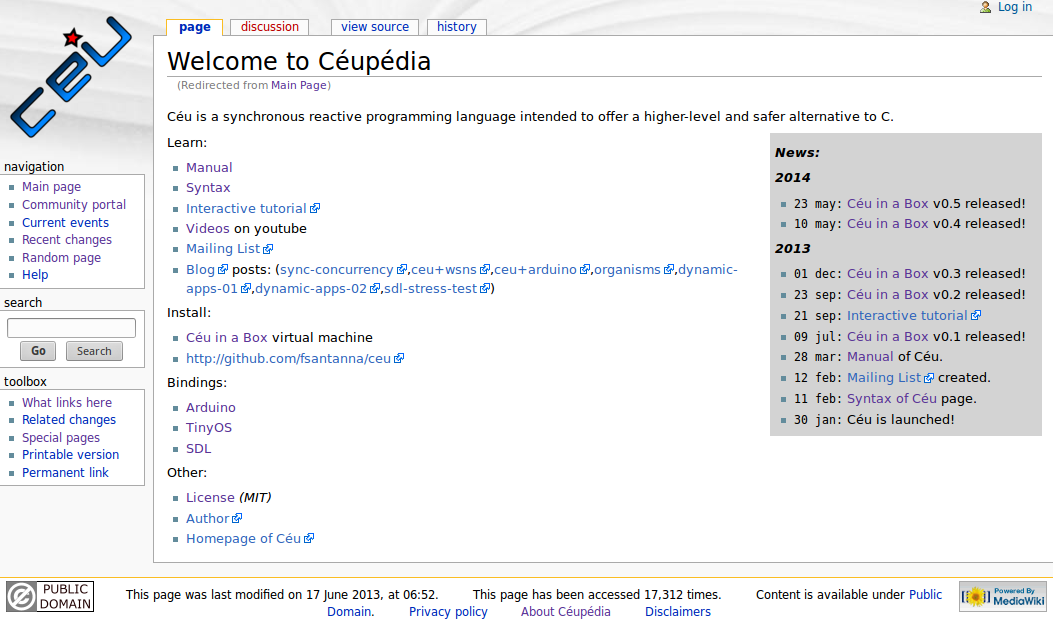
\includegraphics[scale=0.37]{wiki.png}
\rule{14cm}{0.37pt}
\caption{ C\'eup\'edia, the wiki-page of \CEU.
\label{fig.wiki}
}
\end{figure}

\begin{figure}[t]
\centering
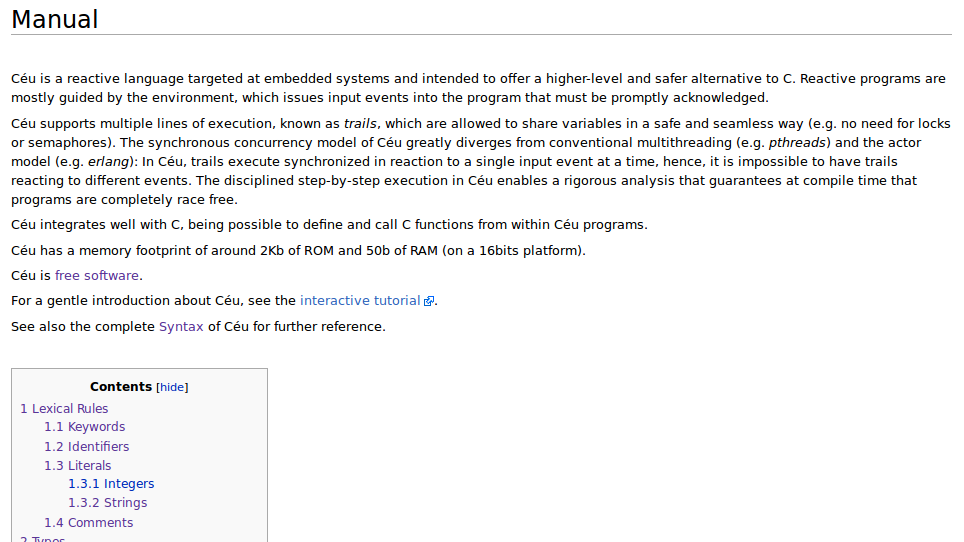
\includegraphics[scale=0.35]{manual.png}
\rule{14cm}{0.45pt}
\caption{ Online manual of \CEU.
\label{fig.wiki}
}
\end{figure}

\begin{figure}[t]
\centering
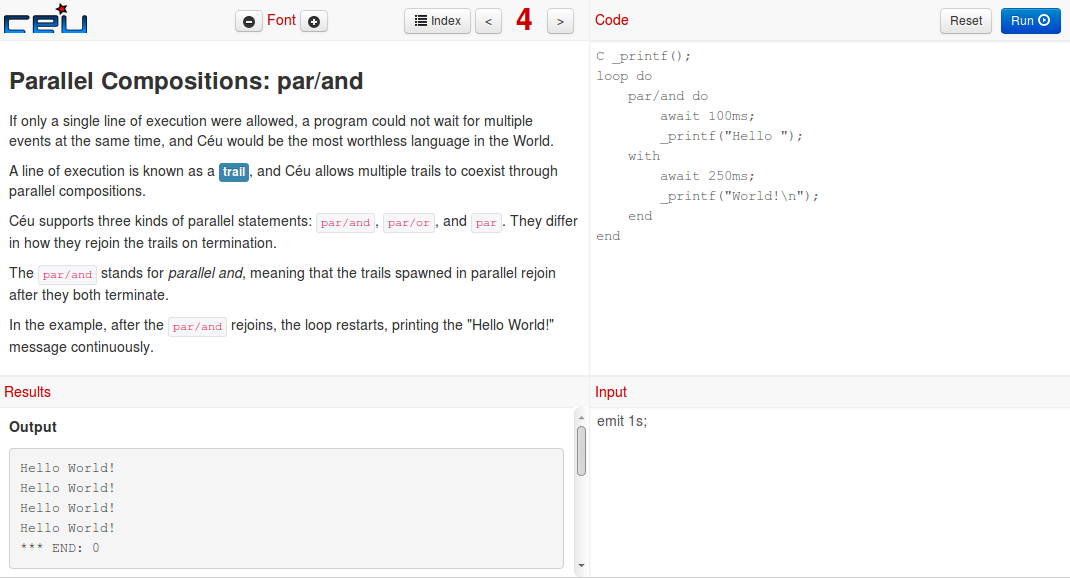
\includegraphics[scale=0.35]{tutorial.png}
\rule{14cm}{0.37pt}
\caption{ Online-interactive tutorial on \CEU. (Thanks to Carlos Mattoso)
\label{fig.tutorial}
}
\end{figure}

\begin{figure}[t]
\centering
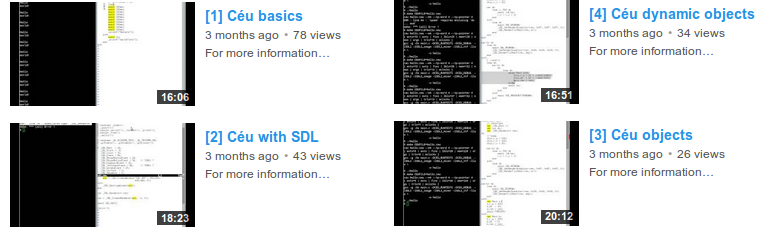
\includegraphics[scale=0.48]{videos.png}
\rule{14cm}{0.37pt}
\caption{ Introductory videos about \CEU.
\label{fig.videos}
}
\end{figure}

\begin{figure}[t]
\centering
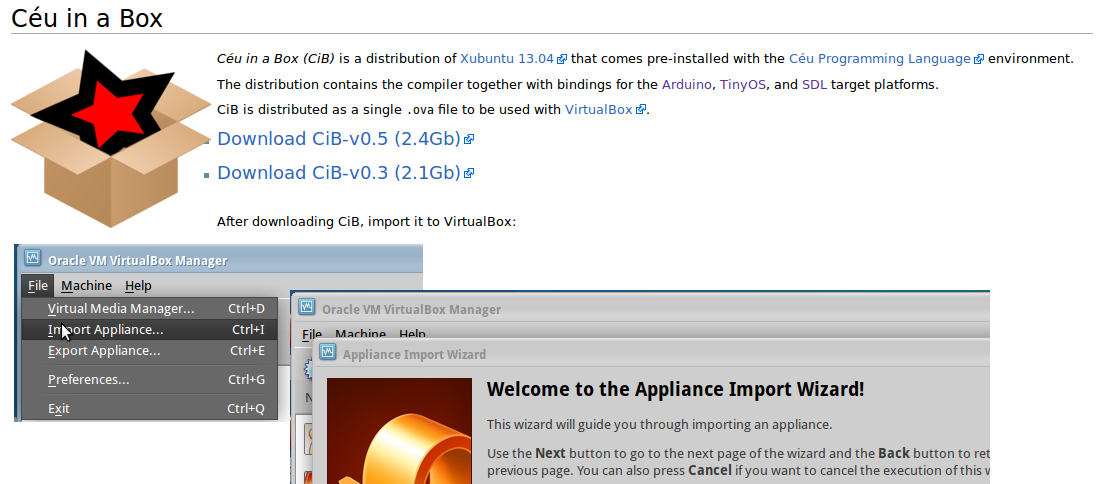
\includegraphics[scale=0.35]{cib.png}
\rule{14cm}{0.37pt}
\caption{ ``C\'eu-in-a-box'': a linux-based VM pre-installed with \CEU for 
TinyOS, Arduino, and SDL.
\label{fig.cib}
}
\end{figure}

\subsection{Classes}
    - puc, ufrj, ort
    - after nesC, they rapidly recognize the gains in productivity with await
